We used the FLORIS wake model to predict the wind speeds throughout the wind farms in our study\cite{gebraad2016wind}. The FLORIS model is similar to the Jensen wake model used in many wind farm studies\cite{jensen1983note} in that it is a reduced order model well suited for optimization studies in which there will be many calls to the wake model. However, unlike the Jensen wake model which defines one wind speed across an entire wake, FLORIS defines three separate velocity zones, better capturing the physics in a wake. These two wake models are shown in Figure \ref{wake_models}.
%I don't know how it will look on paper, but I can barely see the third wake zone in the FLORIS model. It looks almost white.

\begin{figure}[htbp]
  \centering
  \subfloat[Jensen wake model.]{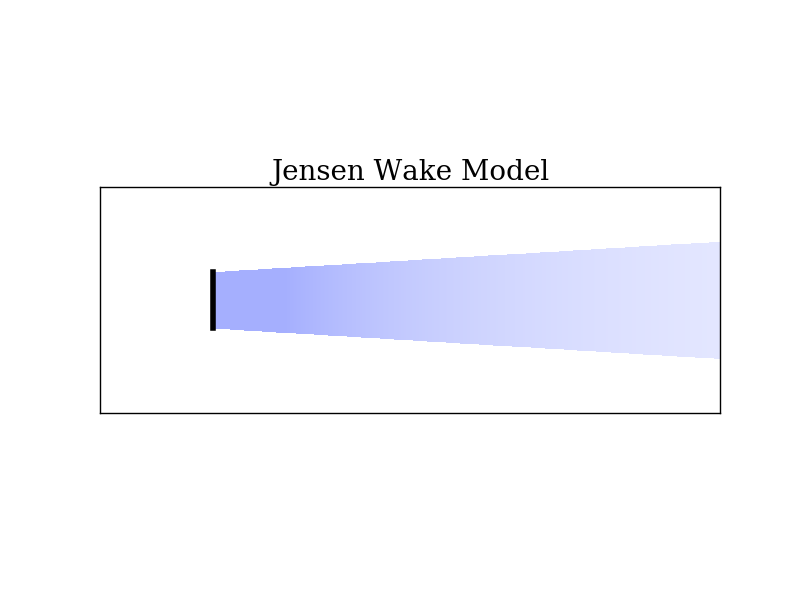
\includegraphics[width=0.5\textwidth]{Figures/Jensen.png}\label{jensen}}
  \subfloat[FLORIS wake model.]{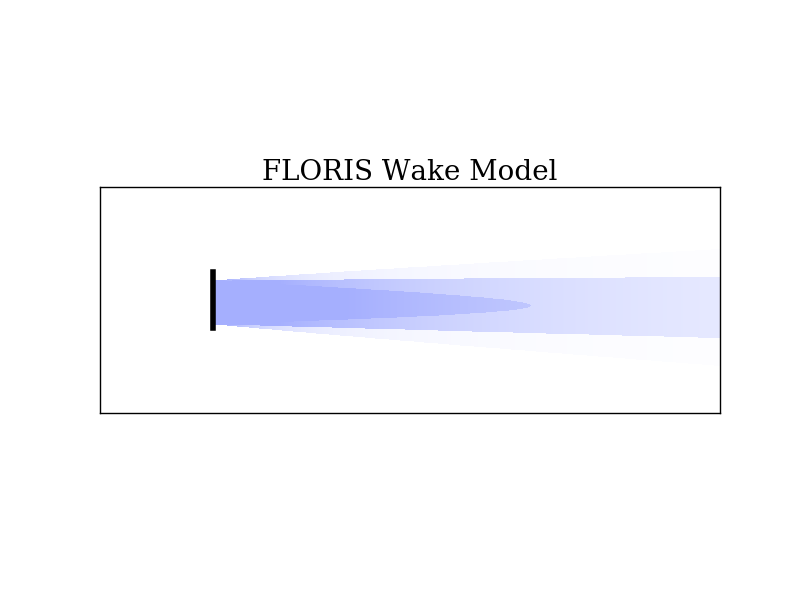
\includegraphics[width=0.5\textwidth]{Figures/Floris.png}\label{floris}}
  \caption{\label{wake_models} The Jensen and FLORIS wake models. Notice the three separate wake zones captured in the FLORIS wake model, and the single wake zone in the Jensen model.}
\end{figure}

The FLORIS model had some discontinuities in the original formulation. In this study we use a version that has been modified to be smooth and continuously differentiable\cite{thomas2017improving}, enabling gradient-based optimization.
%Check your citations for what type of style manual you are using (Chicago, APA, etc.) For most style manuals, all footnotes go at the end of the sentence.

The total wake deficit at any given point is defined as the square root of the sum of the squares of the loss contribution from each turbine wake:

\begin{equation}
L = \sqrt{\sum_{i=1}^\text{nTurbs}L_i^2}
\end{equation}

\noindent Thus at any point in the wind farm, the wind speed is:

\begin{equation}
V = V_\infty(1-L)
\end{equation}

\noindent Note that $V_\infty$ is defined as the freestream wind speed at the hub height of the wind turbine in question. Variations of the freestream wind speed are calculated with the wind profile power law: 
\begin{equation}
V = V_{\text{ref}}\Big(\frac{z}{z_{\text{ref}}}\Big)^\alpha
\label{Eq:shear}
\end{equation}
where $V_{\text{ref}}$ is the reference wind speed given by the wind data, $z_{\text{ref}}$ is height at which the reference wind speed was measured, which we assumed to be 50 meters, $V$ is the wind speed at and height $z$, and $\alpha$ is the wind shear exponent, which defines how the wind speed varies with height.